\documentclass[12pt,a4paper,french]{article}
\usepackage[utf8]{inputenc}
\usepackage{babel}
\usepackage[T1]{fontenc}
\usepackage{dsfont}
\usepackage{amsmath}
\usepackage[top=1cm,bottom=1cm,left=1.5cm, right=1.5cm]{geometry}
\usepackage{tcolorbox}
\usepackage{parskip}
\usepackage{graphicx}
\usepackage{float}
\usepackage{tikz,tkz-tab}
\usepackage{appendix}
\usepackage{tabularx}
\usepackage{amsmath}
\usepackage{rotating}
\usepackage{esvect}
\usepackage{cancel}
\usetikzlibrary{positioning}
\usepackage{pgfpages}
\usepackage{multicol}
\usepackage{tkz-euclide}
\usepackage{esvect}
\usepackage{enumerate}
\usepackage{fancyhdr}
\usepackage{lipsum}
\usepackage{amssymb}
\usepackage{diagbox}
\usepackage[nomessages]{fp}
\usepackage{svg}

%\pgfpagesuselayout{2 on 1}[a4paper,landscape]\pgfpageslogicalpageoptions{1}{border code=\pgfusepath{stroke}}\pgfpageslogicalpageoptions{2}{border code=\pgfusepath{stroke}} %2 en 1

\AtBeginDocument{\renewcommand\labelitemi{$\bullet$}}%Itemize avec des bullet !


\advance\year by -1
\ifnum \the\month > 7 \advance\year by 1 \fi %pour la bonne année en bas à droite 

\newcommand\nextyear
{\advance\year by 1 \the\year\advance\year by -1}

\pagestyle{fancy}
\fancyhf{}
\renewcommand{\headrulewidth}{0pt}
% \fancyfoot[LO,RE]{M. Loizon}
% \fancyfoot[RO,LE]{\the\year /\nextyear}
% \fancypagestyle{plain}{
%   \fancyfoot[C]{\thepage}% you can add edits that won't affect "fancy" but only "plain"
% }

\hyphenpenalty 10000
\exhyphenpenalty 10000

\graphicspath{ {./Images/} }

%%%%%%%%%%%%%%%%%%%%%%%%%%%%%%%%%%%%%    AIDE    %%%%%%%%%%%%%%%%%%%%%%%%%%%%%%
%\refstepcounter{propcntr}\label{chgtdnmntr}\addtocounter{propcntr}{-1} %Ref to counter


%%%%%%%%%%%%%%%%%%%%%%%%%%%%%%%%%%%%% COMMANDES %%%%%%%%%%%%%%%%%%%%%%%%%%%%%%%


\newcommand*{\zz}{\mathds{Z}}

\newcommand*{\nn}{\mathds{N}}

\newcommand*{\qq}{\mathds{Q}}

\newcommand*{\rr}{\mathds{R}}

\newcolumntype{Y}{>{\centering\arraybackslash}X}

\newcounter{propcntr}%PROPRIETE
    \newtcolorbox{propriete}[1]{colback=white,colframe=gray,fonttitle=\bfseries,title=\stepcounter{propcntr} Propriété~\arabic{propcntr}~: \MakeUppercase#1}%Boite propriétés

\newcounter{defcntr}%Définition
    \newtcolorbox{definition}[1]{colback=white,colframe=lightgray,fonttitle=\bfseries,title=\stepcounter{propcntr} Définition~\arabic{propcntr}~: \MakeUppercase#1}%Boite definition

\newif\ifshowcours%Pour cacher le cours
    \showcoursfalse
    \newcommand{\cours}[1]{\ifshowcours #1 \fi}
\showcourstrue%Montre le cours

\newcounter{exmplcntr}%Exemple
    \newcommand*{\exmpl}[1]{\stepcounter{exmplcntr}{\cours{\textbf{Exemple~\arabic{exmplcntr}~:~} #1}
    \medskip}}%sans liste

\newcommand{\rmq}[1]{\cours{\textbf{Remarque~:~}#1}}%Remarque

\newcommand*{\prop}[2]{
        \begin{propriete}{#1}
            #2
        \end{propriete}
        }
   
\newcommand*{\dfnt}[2]{
    \begin{definition}{#1}
        #2
    \end{definition}
    }

\newcounter{excntr}%(a)
    \newcommand*{\cnt}{\stepcounter{excntr}{(\alph{excntr})~~}}

\begin{document}

\renewcommand{\arraystretch}{3}

\newcommand{\titre}
{Chapitre 1 : Géométrie dans l'espace }

%Place dans un tableau

\rhead{Devoir n° 1 du 29 Septembre 2023}


\lhead{Nom, prénom :}

\exo{4}{Calculer} Calculer en détaillant les étapes

\begin{multicols}{2}
    $$-13-14$$
    \vspace*{3em}

    $$-12+21$$
    \vspace*{7em}\columnbreak

    $$-6+4-12+2$$
    \vspace*{3em}

    $$-12+11-14+20+3$$
    \vspace*{7em}
\end{multicols}

\vspace*{-1em}

\exo{4}{Calculer} Calculer en détaillant les étapes

\begin{multicols}{2}
    $$(+12)+(-11)+(-6)+(+1)$$
    \vspace*{8em}

    $$(-10)-(-5)+(-8)-(+5)$$
    \vspace*{8em}\columnbreak

    $$(-1)-(-1)+(-6)+(-1)-(+8)-(-5)$$
    \vspace*{8em}

    $$(+6)-(+3)-(-8)-(+4)-(-3)-(+6)$$
    \vspace*{8em}
\end{multicols}

\newpage



\exo{4}{Chercher} Trouve les erreurs :

\begin{multicols}{2}
    \noindent\begin{align*}
        &(+10)+(-6)-(+2)-(-12)\\
        =&+10-6-2-12\\
        =&+10-20\\
        =&-10
    \end{align*}

    \noindent\begin{align*}
        &(-13)-(-4)-(+5)+(+9)\\
        =&-13+4-5+9\\
        =&-18+13\\
        =&+5
    \end{align*}

\end{multicols}

\exo{4}{Modéliser} Résoudre les problèmes suivants :

\begin{minipage}{0.45\textwidth}
    Crabe et Goyle jouent à un jeu de société. Crabe a 12 points et Goyle en a 27.
    Crabe lui échange un jeton valant -5 points contre un jeton en valant +3. 
    Qui a le plus de point désormais ?
    \vspace*{8em}
\end{minipage}
\hfil
\vrule
\hfil
\begin{minipage}{0.45\textwidth}
    Crabe et Goyle jouent à un jeu de société. Crabe a -12 points et Goyle en a -1.
    Crabe lui échange un jeton valant -4 points contre un jeton en valant +1. 
    Qui a le plus de point désormais ?
    \vspace*{8em}
\end{minipage}

\exo{4}{Raisonner} Simplifier les écritures suivantes.

\begin{multicols}{2}
    $$-(+(-5))$$
    \vspace*{3em}

    $$-(-(+(-7)))$$
    \vspace*{7em}\columnbreak

    $$+(+(-1))$$
    \vspace*{3em}

    $$+(-(-(+2)))$$
    \vspace*{7em}
\end{multicols}

\exo{}{Calculer}

$$6\times 5 -(-4-(-2))\times 3 +((9\times 4)-(-6))\div 7+\noindent4-(+12)$$


\newpage

\setcounter{exrcntr}{0}

\exrc (4 points) Effectuer les calculs suivants

\begin{tabularx}{\textwidth}{Y|Y}
    \cnt  & \cnt  \\
    $3+5\times 7 -3+1$ & $4+5\times (6-3+2)$
\end{tabularx} 

\exrc (2 points) Compléter le tableau suivant \textbf{(peut être fait sur le sujet)}.

\begin{tabularx}{\textwidth}{Y|Y}
    Forme décimale & Forme pourcentage \\ \hline
    & 35\% \\ \hline
    0,65 & \\ \hline
    & 9\% \\ \hline
    0,8 & 
\end{tabularx} 

\exrc (4 points) A l'aide du diagrame ci dessous.

\begin{figure}[H]
    \centering
    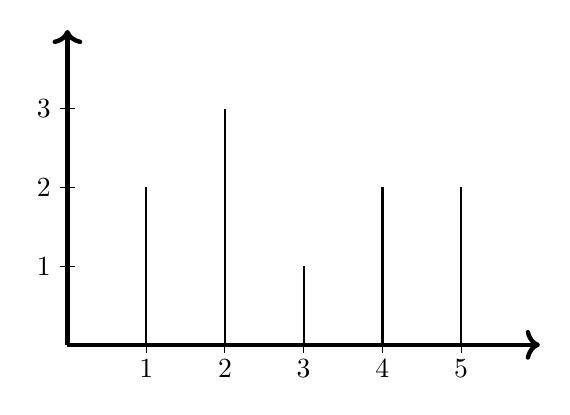
\begin{tikzpicture}
    \draw[ultra thick,->] (0,0)--(6,0) ; 
    \draw[ultra thick,->] (0,0) -- (0,4) ; 
    \foreach \r in {1,...,5}{\draw[color=black] (\r , -0.1)--(\r , 0.1);
    \draw (\r , -0.3) node {\r} ;}
    \foreach \r in {1,...,3}{\draw[color=black] (-0.1,\r )--( 0.1, \r);
    \draw (-0.3 , \r) node {\r} ;}
    \draw[thick] (1,0) -- (1,2) ;
    \draw[thick] (2,0) -- (2,3) ;
    \draw[thick] (3,0) -- (3,1) ;
    \draw[thick] (4,0) -- (4,2) ;
    \draw[thick] (5,0) -- (5,2) ;
    \end{tikzpicture}
    \end{figure}

\cnt (2 points) Compléter le tableau d'effectif \textbf{(peut être fait sur le sujet)}.

\begin{tabularx}{\textwidth}{Y*{5}{|Y}}
    Valeur &  1 & 2 & 3 & 4 & 5\\ \hline
    Effectif &  &  &  & &
\end{tabularx} 

\cnt (1 point) Calculer la fréquence de la valeur 5.

\cnt (1 point) Calculer la fréquence de la valeur 3.

\newpage

\exrc (5 points) Calculer les moyennes des séries suivantes

\cnt (2 points) 1 ; 2 ; 3 ; 4 ; 10 

\cnt (2 points) 5 ; 11 ; 14 ; 8 ; 13 ; 9

\cnt (1 points) la série définie par le tableau suivant :

\begin{tabularx}{\textwidth}{Y*{4}{|Y}}
    Valeur &  2 & 4 & 5 & 10\\ \hline
    Effectif & 3 & 1 & 2 & 4
\end{tabularx} 

\exrc (5 points) Calculer les médianes des séries suivantes

\cnt (2 points) 1 ; 2 ; 3 ; 4 ; 5 

\cnt (2 points) 12 ; 13 ; 7 ; 5 ; 1 ; 2

\cnt (1 points) la série définie par le tableau suivant :

\begin{tabularx}{\textwidth}{Y*{5}{|Y}}
    Valeur &  12 & 15  & 19 & 25 & 39\\ \hline
    Effectif & 2 & 1 & 1 & 4 & 3
\end{tabularx} %Mode préparation

%\section*{\titre- Correction}

\begin{minipage}[t]{0.23\textwidth}
    \exo{Chercher}{CarreMagique1}
    \begin{tabularx}{\textwidth}{|Y|Y|Y|}
        \hline
        8 &  6 & -2 \\\hline
        0 & 1 & 11  \\\hline
        4 &  5 & 3 \\\hline
    \end{tabularx}
\end{minipage}
\hfill
\begin{minipage}[t]{0.23\textwidth}
    \exo{Chercher}{CarreMagique2}
    \begin{tabularx}{\textwidth}{|Y|Y|Y|}
        \hline
        5  &  0  & 1  \\\hline
        -2 &  2  & 6  \\\hline
        3  &  4  & -1 \\\hline
    \end{tabularx}
\end{minipage}
\hfill
\begin{minipage}[t]{0.23\textwidth}
    \exo{Chercher}{CarreMagique3}
    \begin{tabularx}{\textwidth}{|Y|Y|Y|}
        \hline
         -1 &  6  & -5 \\\hline
         -4 &  0  & 4 \\\hline
         5 &  -6  & 1 \\\hline
    \end{tabularx}
\end{minipage}
\hfill
\begin{minipage}[t]{0.23\textwidth}
    \exo{Chercher}{CarreMagique4}
    \begin{tabularx}{\textwidth}{|Y|Y|Y|}
        \hline
         -16 & -1 & -4  \\\hline
         5 & -7 &  -19 \\\hline
        -10& -13& 2  \\\hline
    \end{tabularx}
\end{minipage}

%Pour avoir les corrigés

% \section*{Chapitre 2 : Symétries centrales - Plan de Travail}

\pdt[]{Rappel : Symétrie axiale}
{\begin{multicols}{4}
\begin{itemize}
    \itemindent=-25pt
        \item \exref{TracerSymAxQuadri1}
        \item \exref{TracerSymAxQuadri2}
        \item \exref{TracerSymAxQuadri3}
        \item \exref{TracerSymAxQuadri4}
        \item \exref{TracerSymAxBlanc1}
        \item \exref{TracerSymAxBlanc2}
        \item \exref{TracerSymAxBlanc3}
        \item \exref{TracerSymAxBlanc4}
        \item \exref{CentreSymAx1}
        \item \exref{CentreSymAx2}
        \item \exref{CentreSymAx3}
        \item \exref{CentreSymAx4}
    \end{itemize}
\end{multicols}}

\begin{plandetravailDS}
    Programme de l'interro :
    \begin{itemize}
        \item Revoir chapitre 1 : faire un calcul avec priorité (2 points) 
        \item Faire une symétrie sans quadrillage (2 points)
        \item Faire une symétrie avec quadrillage (4 points)
        \item Retrouver le centre d'une symétrie (2 points)
    \end{itemize}
\end{plandetravailDS}

\begin{minipage}[t]{0.5\textwidth}
    \pdt[6]{Symétrie centrale avec quadrillage}
    {\begin{multicols}{2}
    \begin{itemize}
        \itemindent=-25pt
            \item \exref{TracerSymCentQuadri1}
            \item \exref{TracerSymCentQuadri2}
            \item \exref{TracerSymCentQuadri3}
            \item \exref{TracerSymCentQuadri4}
            \item \exref{TracerSymCentQuadri5}
            \item \exref{TracerSymCentQuadri6}
            \item \exref{TracerSymCentQuadri7}
            \item \exref{TracerSymCentQuadri8}
        \end{itemize}
    \end{multicols}}
\end{minipage}
\hfill
\begin{minipage}[t]{0.5\textwidth}
    \pdt[4]{Symétrie centrale sans quadrillage}
    {\begin{multicols}{2}
    \begin{itemize}
        \itemindent=-25pt
            \item \exref{TracerSymCentBlanc1}
            \item \exref{TracerSymCentBlanc2}
            \item \exref{TracerSymCentBlanc3}
            \item \exref{TracerSymCentBlanc4}
            \item \exref{TracerSymCentBlanc5}
            \item \exref{TracerSymCentBlanc6}
            \item \exref{TracerSymCentBlanc7}
            \item \exref{TracerSymCentBlanc8}
        \end{itemize}
    \end{multicols}}
\end{minipage}

\pdt[4]{Retrouver le centre d'une symétrie}{
    \begin{multicols}{4}
        \begin{itemize}
            \itemindent=-25pt
                \item \exref{CentreSymCent1}
                \item \exref{CentreSymCent2}
                \item \exref{CentreSymCent3}
                \item \exref{CentreSymCent4}
                \item \exref{CentreSymCent5}
                \item \exref{CentreSymCent6}
                \item \exref{CentreSymCent7}
                \item \exref{CentreSymCent8}
            \end{itemize}
    \end{multicols}
}


\vspace{-1em}

\begin{minipage}[t]{0.5\textwidth}
    \vspace{-0.25em}
    \pdt[1]{Exercices plus difficiles}{
        \begin{multicols}{2}
            \begin{itemize}
                \itemindent=-25pt
                \item \exref{Dur1}
                \item \exref{Dur2}
            \end{itemize}
        \end{multicols}
    }
\end{minipage}  
\hfill
\begin{minipage}[t]{0.47\textwidth}
    \vspace{-0.25em}
    \textbf{Que mettre dans les cases ?}
    \begin{itemize}
        \item \textbf{TB} \textit{(Très bien)} Si tout est juste
        \item \textbf{B} \textit{(Bien)} J'ai le bon résultat, mais pas la bonne rédaction
        \item \textbf{AB} \textit{(Assez bien)} J'ai une faute, mais je peux comprendre avec la correction
        \item  \textbf{AA} \textit{(Avec de l'Aide)} Si j'ai eu besoin d'aide pour réussir l'exercice 
        \item \textbf{A} \textit{(Au secours!)} J'ai besoin que quelqu'un m'explique.
    \end{itemize}
\end{minipage}

% \newpage
% \pgfpagesuselayout{2 on 1}[a4paper,landscape]\pgfpageslogicalpageoptions{1}{border code=\pgfusepath{stroke}}\pgfpageslogicalpageoptions{2}{border code=\pgfusepath{stroke}}%2 en 1

\newpage

\section*{Chapitre 2 : Les symétries centrales - Exercices}

\textbf{Pour les exercies \ref{TracerSymAxQuadri1} à \ref{TracerSymAxQuadri4} :} Tracer l'image de la figure suivante par la symétrie d'axe $(d)$.

\vspace{-2em}
\begin{minipage}[t]{0.45\textwidth}
    \exo{Représenter}{TracerSymAxQuadri1}
    
    \begin{figure}[H]
        \centering
        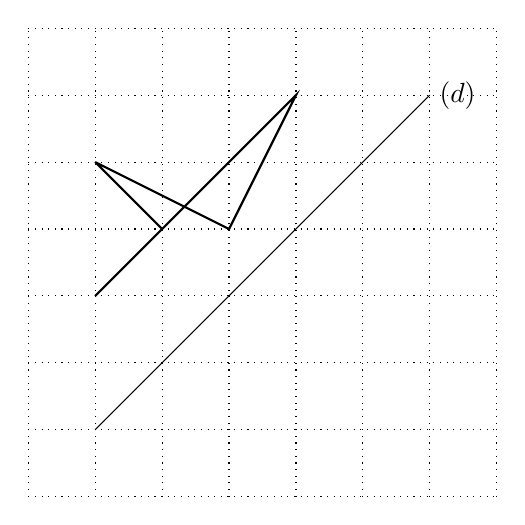
\begin{tikzpicture}[scale=0.85]
            \def\mypath{(-2,2) -- (-1,1) --(-2,0) -- (1,3)--(0,1)--(-2,2)}
            \draw [thick]\mypath ;
            \draw (-2,-2)--(3,3) node [right]{$(d)$} ;
            % \draw [cm={0,1,1,0,(0,0)}] \mypath;%Matrice de transformation inverse X et Y
            \draw [dotted](-3,-3) grid (4,4);
        \end{tikzpicture}
    \end{figure}
\end{minipage}
\hfill
\begin{minipage}[t]{0.45\textwidth}
    \exo{Représenter}{TracerSymAxQuadri2}
    
    \begin{figure}[H]
        \centering
        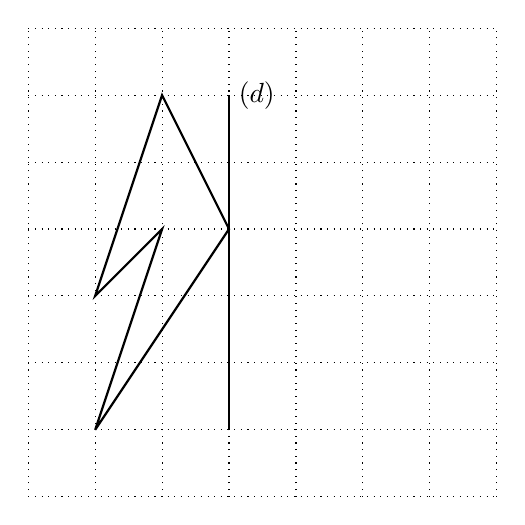
\begin{tikzpicture}[scale=0.85]
            \def\mypath{(-2,-2) -- (-1,1) --(-2,0) -- (-1,3)--(0,1)--(-2,-2)}
            \draw [thick]\mypath ;
            \draw (0,-2)--(0,3) node [right]{$(d)$} ;
            % \draw [cm={-1,0,0,1,(0,0)}] \mypath;%Matrice de transformation inverse X et Y
            \draw [dotted](-3,-3) grid (4,4);
        \end{tikzpicture}
    \end{figure}
\end{minipage}
\vspace{-1em}
\begin{minipage}[t]{0.45\textwidth}
    \exo{Représenter}{TracerSymAxQuadri3}
    
    \begin{figure}[H]
        \centering
        \begin{tikzpicture}[scale=0.85]
            \def\mypath{(-2,-2) -- (0,-1) --(3,-2) -- (2,0)--(-1,-1)--(-2,-2)}
            \draw [thick]\mypath ;
            \draw (-2,0)--(3,0) node [right]{$(d)$} ;
            % \draw [cm={1,0,0,-1,(0,0)}] \mypath;%Matrice de transformation inverse X et Y
            \draw [dotted](-3,-3) grid (4,4);
        \end{tikzpicture}
    \end{figure}
\end{minipage}
\hfill
\begin{minipage}[t]{0.45\textwidth}
    \exo{Représenter}{TracerSymAxQuadri4}
    
    \begin{figure}[H]
        \centering
        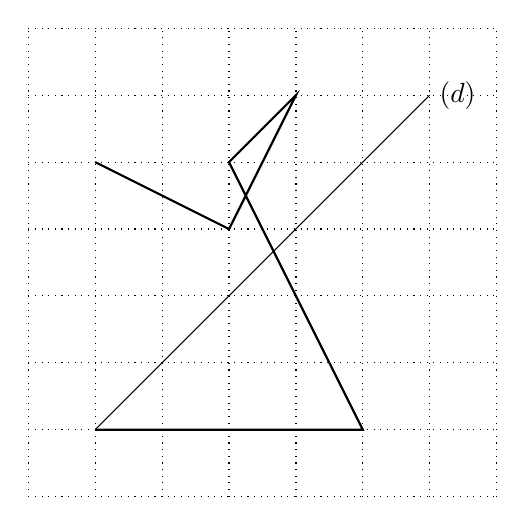
\begin{tikzpicture}[scale=0.85]
            \def\mypath{(-2,-2) -- (2,-2) --(0,2) -- (1,3)--(0,1)--(-2,2)}
            \draw [thick]\mypath ;
            \draw (-2,-2)--(3,3) node [right]{$(d)$} ;
            % \draw [cm={0,1,1,0,(0,0)}] \mypath;%Matrice de transformation inverse X et Y
            \draw [dotted](-3,-3) grid (4,4);
        \end{tikzpicture}
    \end{figure}
\end{minipage}

\vspace{2em}
\textbf{Pour les exercices \ref{TracerSymCentQuadri1} à \ref{TracerSymCentQuadri4} :} Tracer l'image de la figure suivante par la symétrie de centre $O$.
\vspace{-2em}

\begin{minipage}[t]{0.45\textwidth}
    \exo{Représenter}{TracerSymCentQuadri1}
    
    \begin{figure}[H]
        \centering
        \begin{tikzpicture}[scale=0.85]
            \tikzset{
                homothety at/.style args={#1 scaled by #2}{shift={($(#1)!#2!(0,0)$)},scale=#2},}
            \def\mypath{(-2,2) -- (-1,1) --(-2,0) -- (1,3)--(0,1)--(-2,2)}
            \draw [thick]\mypath ;
            \fill (0,0) coordinate (c) circle(2pt) node [above] {$O$};
            % \begin{scope}[homothety at=c scaled by -1]
            %     \draw \mypath;
            % \end{scope}
            \draw [dotted](-3,-3) grid (4,4);
        \end{tikzpicture}
    \end{figure}
\end{minipage}
\hfill
\begin{minipage}[t]{0.45\textwidth}
    \exo{Représenter}{TracerSymCentQuadri2}
    
    \begin{figure}[H]
        \centering
        \begin{tikzpicture}[scale=0.85]
            \tikzset{
                homothety at/.style args={#1 scaled by #2}{shift={($(#1)!#2!(0,0)$)},scale=#2},}
            \def\mypath{(-2,-2) -- (-1,1) --(-2,0) -- (-1,3)--(0,1)--(-2,-2)}
            \draw [thick]\mypath ;
            \fill (1,0) coordinate (c) circle(2pt) node [above] {$O$};
            % \begin{scope}[homothety at=c scaled by -1]
            %     \draw \mypath;
            % \end{scope}
            \draw [dotted](-3,-3) grid (4,4);
        \end{tikzpicture}
    \end{figure}
\end{minipage}

\begin{minipage}[t]{0.45\textwidth}
    \exo{Représenter}{TracerSymCentQuadri3}
    
    \begin{figure}[H]
        \centering
        \begin{tikzpicture}[scale=0.85]
            \tikzset{
                homothety at/.style args={#1 scaled by #2}{shift={($(#1)!#2!(0,0)$)},scale=#2},}
            \def\mypath{(-2,-2) -- (0,-1) --(3,-2) -- (2,0)--(-1,-1)--(-2,-2)}
            \draw [thick]\mypath ;
            \fill (0,0) coordinate (c) circle(2pt) node [above] {$O$};
            % \begin{scope}[homothety at=c scaled by -1]
            %     \draw \mypath;
            % \end{scope}
            \draw [dotted](-3,-3) grid (4,4);
        \end{tikzpicture}
    \end{figure}
\end{minipage}
\hfill
\begin{minipage}[t]{0.45\textwidth}
    \exo{Représenter}{TracerSymCentQuadri4}
    
    \begin{figure}[H]
        \centering
        \begin{tikzpicture}[scale=0.85]
            \tikzset{
                homothety at/.style args={#1 scaled by #2}{shift={($(#1)!#2!(0,0)$)},scale=#2},}
            \def\mypath{(-2,-2) -- (2,-2) --(0,2) -- (1,3)--(0,1)--(-2,2)}
            \draw [thick]\mypath ;
            \fill (0,1) coordinate (c) circle(2pt) node [above] {$O$};
            % \begin{scope}[homothety at=c scaled by -1]
            %     \draw \mypath;
            % \end{scope}
            \draw [dotted](-3,-3) grid (4,4);
        \end{tikzpicture}
    \end{figure}
\end{minipage}

\textbf{Pour l'exercice \ref{TracerTransQuadri1} à \ref{TracerTransQuadri4} :} Tracer l'image de la figure suivante par la translation qui envoie $A$ en $B$.
\vspace{-2em}

\begin{minipage}[t]{0.45\textwidth}
    \exo{Représenter}{TracerTransQuadri1}
    
    \begin{figure}[H]
        \centering
        \begin{tikzpicture}[scale=0.85]
            \def\mypath{(-2,2) -- (-1,1) --(-2,0) -- (1,3)--(0,1)--(-2,2)}
            \draw [thick]\mypath;
            % \draw [shift={(1,-3)}]\mypath ;
            \fill (2,3) coordinate (c) circle(2pt) node [above] {$A$};
            \fill (3,0) coordinate (c) circle(2pt) node [above] {$B$};
            \draw [dotted](-3,-3) grid (4,4);
        \end{tikzpicture}
    \end{figure}
\end{minipage}
\hfill
\begin{minipage}[t]{0.45\textwidth}
    \exo{Représenter}{TracerTransQuadri2}
    
    \begin{figure}[H]
        \centering
        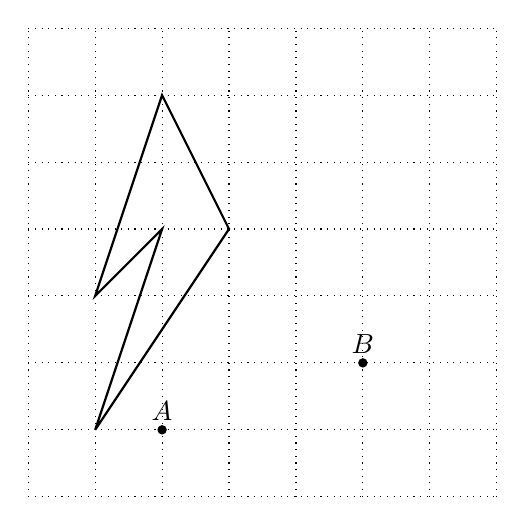
\begin{tikzpicture}[scale=0.85]
            \def\mypath{(-2,-2) -- (-1,1) --(-2,0) -- (-1,3)--(0,1)--(-2,-2)}
            \draw [thick]\mypath;
            % \draw [shift={(3,1)}]\mypath ;
            \fill (-1,-2) coordinate (c) circle(2pt) node [above] {$A$};
            \fill (2,-1) coordinate (c) circle(2pt) node [above] {$B$};
            \draw [dotted](-3,-3) grid (4,4);
        \end{tikzpicture}
    \end{figure}
\end{minipage}

\begin{minipage}[t]{0.45\textwidth}
    \exo{Représenter}{TracerTransQuadri3}
    
    \begin{figure}[H]
        \centering
        \begin{tikzpicture}[scale=0.85]
            \def\mypath{(-2,-2) -- (0,-1) --(3,-2) -- (2,0)--(-1,-1)--(-2,-2)}
            \draw [thick]\mypath;
            % \draw [shift={(1,3)}]\mypath ;
            \fill (-1,0) coordinate (c) circle(2pt) node [above] {$A$};
            \fill (0,3) coordinate (c) circle(2pt) node [above] {$B$};
            \draw [dotted](-3,-3) grid (4,4);
        \end{tikzpicture}
    \end{figure}
\end{minipage}
\hfill
\begin{minipage}[t]{0.45\textwidth}
    \exo{Représenter}{TracerTransQuadri4}
    
    \begin{figure}[H]
        \centering
        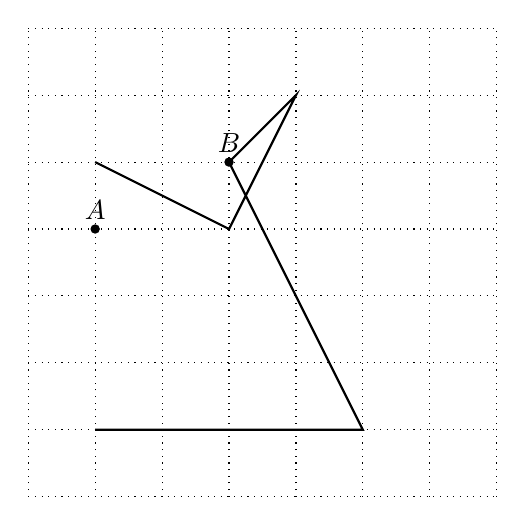
\begin{tikzpicture}[scale=0.85]
            \def\mypath{(-2,-2) -- (2,-2) --(0,2) -- (1,3)--(0,1)--(-2,2)}
            \draw [thick]\mypath;
            % \draw [shift={(2,1)}]\mypath ;
            \fill (-2,1) coordinate (c) circle(2pt) node [above] {$A$};
            \fill (0,2) coordinate (c) circle(2pt) node [above] {$B$};
            \draw [dotted](-3,-3) grid (4,4);
        \end{tikzpicture}
    \end{figure}
\end{minipage}
\newpage

\textbf{Pour les exercices \ref{TracerRotaQuadri1} à \ref{TracerRotaQuadri4} :} Tracer l'image par la rotation de centre $0$ avec l'angle donné.
\vspace{-2em}

\begin{minipage}[t]{0.45\textwidth}
    \exo{Représenter}{TracerRotaQuadri1}
    
    Angle $90$° dans le sens horairere.
    
    \begin{figure}[H]
        \centering
        \begin{tikzpicture}[scale=0.85]
            \def\mypath{(-2,2) -- (-1,1) --(-2,0) -- (1,3)--(0,1)--(-2,2)}
            \draw [thick]\mypath ;
            \fill (0,0) coordinate (c) circle(2pt) node [above] {$0$};
            % \draw [rotate=-90] \mypath ;
            \draw [dotted](-3,-3) grid (4,4);
        \end{tikzpicture}
    \end{figure}
\end{minipage}
\hfill
\begin{minipage}[t]{0.45\textwidth}
    \exo{Représenter}{TracerRotaQuadri2}
    
    Angle $90$° dans le sens anti-horairere.
    
    \begin{figure}[H]
        \centering
        \begin{tikzpicture}[scale=0.85]
            \def\mypath{(-2,-2) -- (-1,1) --(-2,0) -- (-1,3)--(0,1)--(-2,-2)}
            \draw [thick]\mypath ;
            \fill (0,0) coordinate (c) circle(2pt) node [above] {$0$};
            % \draw [rotate=90] \mypath ;
            \draw [dotted](-3,-3) grid (4,4);
        \end{tikzpicture}
    \end{figure}
\end{minipage}
\vspace*{-0.5em}
\begin{minipage}[t]{0.45\textwidth}
    \exo{Représenter}{TracerRotaQuadri3}
    
    Angle $90$° dans le sens horairere.
    
    \begin{figure}[H]
        \centering
        \begin{tikzpicture}[scale=0.85]
            \def\mypath{(-2,-2) -- (0,-1) --(3,-2) -- (2,0)--(-1,-1)--(-2,-2)}
            \draw [thick]\mypath ;
            \fill (0,0) coordinate (c) circle(2pt) node [above] {$0$};
            % \draw [rotate=-90] \mypath ;
            \draw [dotted](-3,-3) grid (4,4);
        \end{tikzpicture}
    \end{figure}
\end{minipage}
\hfill
\begin{minipage}[t]{0.45\textwidth}
    \exo{Représenter}{TracerRotaQuadri4}
    
    Angle $90$° dans le sens anti-horairere.
    
    \begin{figure}[H]
        \centering
        \begin{tikzpicture}[scale=0.85]
            \def\mypath{(-2,-2) -- (2,-2) --(0,2) -- (1,3)--(0,1)--(-2,2)}
            \draw [thick]\mypath ;
            \fill (0,0) coordinate (c) circle(2pt) node [above] {$0$};
            % \draw [rotate=90] \mypath ;
            \draw [dotted](-3,-3) grid (4,4);
        \end{tikzpicture}
    \end{figure}
\end{minipage}

\textbf{Pour les exercices \ref{TracerHomotQuadri1} à \ref{TracerHomotQuadri4} : }Tracer l'image par l'homothétie de centre $O$ avec le rapport donné.
\vspace{-2em}

\begin{minipage}[t]{0.45\textwidth}
    \exo{Représenter}{TracerHomotQuadri1}
    
    Rapport 2.
    
    \begin{figure}[H]
        \centering
        \begin{tikzpicture}[scale=0.85]
            \tikzset{
                homothety at/.style args={#1 scaled by #2}{shift={($(#1)!#2!(0,0)$)},scale=#2},}
            \def\mypath{(-2,2) -- (-1,1) --(-2,0) -- (1,3)--(0,1)--(-2,2)}
            \draw [thick]\mypath ;
            \fill (-1,2) coordinate (c) circle(2pt) node [above] {$O$};
            % \begin{scope}[homothety at=c scaled by 2]
            %     \draw \mypath;
            % \end{scope}
            \draw [dotted](-3,-3) grid (5,5);
        \end{tikzpicture}
    \end{figure}
\end{minipage}
\hfill
\begin{minipage}[t]{0.45\textwidth}
    \exo{Représenter}{TracerHomotQuadri2}
    
    Rapport 1,5.
    
    \begin{figure}[H]
        \centering
        \begin{tikzpicture}[scale=0.85]
            \tikzset{
                homothety at/.style args={#1 scaled by #2}{shift={($(#1)!#2!(0,0)$)},scale=#2},}
            \def\mypath{(-2,-2) -- (-1,1) --(-2,0) -- (-1,3)--(0,1)--(-2,-2)}
            \draw [thick]\mypath ;
            \fill (0,0) coordinate (c) circle(2pt) node [above] {$O$};
            % \begin{scope}[homothety at=c scaled by 1.5]
            %     \draw \mypath;
            % \end{scope}
            \draw [dotted](-3,-3) grid (5,5);
        \end{tikzpicture}
    \end{figure}
\end{minipage}

\begin{minipage}[t]{0.45\textwidth}
    \exo{Représenter}{TracerHomotQuadri3}
    
    Rapport -2.
    
    \begin{figure}[H]
        \centering
        \begin{tikzpicture}[scale=0.85]
            \tikzset{
                homothety at/.style args={#1 scaled by #2}{shift={($(#1)!#2!(0,0)$)},scale=#2},}
            \def\mypath{(-1,-2) -- (0,-1) --(3,-2) -- (2,0)--(-1,-1)--(-1,-2)}
            \draw [thick]\mypath ;
            \fill (1,-1) coordinate (c) circle(2pt) node [above] {$O$};
            % \begin{scope}[homothety at=c scaled by -2]
            %     \draw \mypath;
            % \end{scope}
            \draw [dotted](-3,-3) grid (5,5);
        \end{tikzpicture}
    \end{figure}
\end{minipage}
\hfill
\begin{minipage}[t]{0.45\textwidth}
    \exo{Représenter}{TracerHomotQuadri4}
    
    Rapport 2.
    
    \begin{figure}[H]
        \centering
        \begin{tikzpicture}[scale=0.85]
            \tikzset{
                homothety at/.style args={#1 scaled by #2}{shift={($(#1)!#2!(0,0)$)},scale=#2},}
            \def\mypath{(-2,-2) -- (2,-2) --(0,2) -- (1,3)--(0,1)--(-2,2)}
            \draw [thick]\mypath ;
            \fill (2,1) coordinate (c) circle(2pt) node [above] {$O$};
            % \begin{scope}[homothety at=c scaled by -0.5]
            %     \draw \mypath;
            % \end{scope}
            \draw [dotted](-3,-3) grid (5,5);
        \end{tikzpicture}
    \end{figure}
\end{minipage}

\textbf{Pour les exercies \ref{TracerSymAxBlanc1} à \ref{TracerSymAxBlanc4} :} Tracer l'image de la figure suivante par la symétrie d'axe $(d)$.

\begin{minipage}[t]{0.45\textwidth}
    \exo{Représenter}{TracerSymAxBlanc1}
    
    \begin{figure}[H]
        \centering
        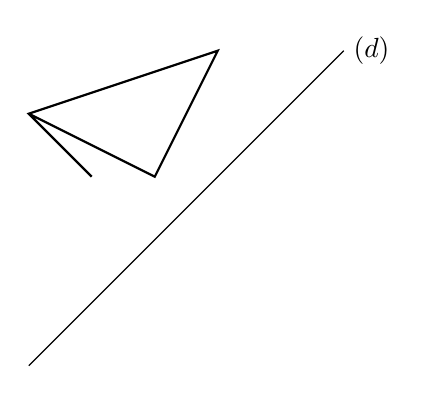
\begin{tikzpicture}[scale=0.8]
            \def\mypath{(-2,2) -- (-1,1) --(-2,2) -- (1,3)--(0,1)--(-2,2)}
            \draw [thick]\mypath ;
            \draw (-2,-2)--(3,3) node [right]{$(d)$} ;
            % \draw [cm={0,1,1,0,(0,0)}] \mypath;%Matrice de transformation inverse X et Y
        \end{tikzpicture}
    \end{figure}
\end{minipage}
\hfill
\begin{minipage}[t]{0.45\textwidth}
    \exo{Représenter}{TracerSymAxBlanc2}
    
    \begin{figure}[H]
        \centering
        \begin{tikzpicture}[scale=0.8]
            \def\mypath{(-2,-2) -- (-1,1) --(-3,0) -- (-1,3)--(1,1)--(-2,-2)}
            \draw [white](-3,-3) grid (4,4);
            \draw [thick]\mypath ;
            \draw (0,-2)--(0,3) node [right]{$(d)$} ;
            % \draw [cm={-1,0,0,1,(0,0)}] \mypath;%Matrice de transformation inverse X et Y 
        \end{tikzpicture}
    \end{figure}
\end{minipage}

\begin{minipage}[t]{0.45\textwidth}
    \exo{Représenter}{TracerSymAxBlanc3}
    
    \begin{figure}[H]
        \centering
        \begin{tikzpicture}[scale=0.8]
            \def\mypath{(1,-2) -- (0,-1) --(3,-2) -- (2,-1)--(-1,-1)--(1,-2)}
            \draw [white](-3,-3) grid (4,4);
            \draw [thick]\mypath ;
            \draw (-2,0)--(3,0) node [right]{$(d)$} ;
            % \draw [cm={1,0,0,-1,(0,0)}] \mypath;%Matrice de transformation inverse X et Y
        \end{tikzpicture}
    \end{figure}
\end{minipage}
\hfill
\begin{minipage}[t]{0.45\textwidth}
    \exo{Représenter}{TracerSymAxBlanc4}
    
    \begin{figure}[H]
        \centering
        \begin{tikzpicture}[scale=0.8]
            \def\mypath{(-2,-1) -- (2,-2) --(1,4) -- (0,1)--(-2,2)}
            \draw [white](-3,-3) grid (4,4);
            \draw [thick]\mypath ;
            \draw (-2,-2)--(3,3) node [right]{$(d)$} ;
            % \draw [cm={0,1,1,0,(0,0)}] \mypath;%Matrice de transformation inverse X et Y
        \end{tikzpicture}
    \end{figure}
\end{minipage}

\textbf{Pour les exercices \ref{TracerSymCentBlanc1} à \ref{TracerSymCentBlanc4} :} Tracer l'image de la figure suivante par la symétrie de centre $O$.

\begin{minipage}[t]{0.45\textwidth}
    \exo{Représenter}{TracerSymCentBlanc1}
    
    \begin{figure}[H]
        \centering
        \begin{tikzpicture}[scale=0.8]
            \tikzset{
                homothety at/.style args={#1 scaled by #2}{shift={($(#1)!#2!(0,0)$)},scale=#2},}
            \def\mypath{(-2,2) -- (-1,1) --(-2,2) -- (1,3)--(0,1)--(-2,2)}
            \draw [white](-3,-3) grid (4,4);
            \draw [thick]\mypath ;
            \fill (0,0) coordinate (c) circle(2pt) node [above] {$O$};
            % \begin{scope}[homothety at=c scaled by -1]
            %     \draw \mypath;
            % \end{scope}
        \end{tikzpicture}
    \end{figure}
\end{minipage}
\hfill
\begin{minipage}[t]{0.45\textwidth}
    \exo{Représenter}{TracerSymCentBlanc2}
    
    \begin{figure}[H]
        \centering
        \begin{tikzpicture}[scale=0.8]
            \tikzset{
                homothety at/.style args={#1 scaled by #2}{shift={($(#1)!#2!(0,0)$)},scale=#2},}
            \def\mypath{(-2,-2) -- (-1,1) --(-3,0) -- (-1,3)--(1,1)--(-2,-2)}
            \draw [white](-3,-3) grid (4,4);
            \draw [thick]\mypath ;
            \fill (1,0) coordinate (c) circle(2pt) node [above] {$O$};
            % \begin{scope}[homothety at=c scaled by -1]
            %     \draw \mypath;
            % \end{scope}
        \end{tikzpicture}
    \end{figure}
\end{minipage}

\begin{minipage}[t]{0.45\textwidth}
    \exo{Représenter}{TracerSymCentBlanc3}
    
    \begin{figure}[H]
        \centering
        \begin{tikzpicture}[scale=0.8]
            \tikzset{
                homothety at/.style args={#1 scaled by #2}{shift={($(#1)!#2!(0,0)$)},scale=#2},}
            \def\mypath{(-2,-2) -- (0,-1) --(3,-2) -- (2,0)--(-1,-1)--(-2,-2)}
            \draw [white](-3,-3) grid (4,4);
            \draw [thick]\mypath ;
            \fill (0,0) coordinate (c) circle(2pt) node [above] {$O$};
            % \begin{scope}[homothety at=c scaled by -1]
            %     \draw \mypath;
            % \end{scope}
        \end{tikzpicture}
    \end{figure}
\end{minipage}
\hfill
\begin{minipage}[t]{0.45\textwidth}
    \exo{Représenter}{TracerSymCentBlanc4}
    
    \begin{figure}[H]
        \centering
        \begin{tikzpicture}[scale=0.8]
            \tikzset{
                homothety at/.style args={#1 scaled by #2}{shift={($(#1)!#2!(0,0)$)},scale=#2},}
            \def\mypath{(-2,-1) -- (2,-2) --(1,4) -- (0,1)--(-2,2)}
            \draw [white](-3,-3) grid (4,4);
            \draw [thick]\mypath ;
            \fill (0,1) coordinate (c) circle(2pt) node [above] {$O$};
            % \begin{scope}[homothety at=c scaled by -1]
            %     \draw \mypath;
            % \end{scope}
        \end{tikzpicture}
    \end{figure}
\end{minipage}

\textbf{Pour l'exercice \ref{TracerTransBlanc1} à \ref{TracerTransBlanc4} :} Tracer l'image de la figure suivante par la translation qui envoie $A$ en $B$.

\begin{minipage}[t]{0.45\textwidth}
    \exo{Représenter}{TracerTransBlanc1}
    
    \begin{figure}[H]
        \centering
        \begin{tikzpicture}[scale=0.8]
            \def\mypath{(-2,2) -- (-1,1) --(-2,2) -- (1,3)--(0,1)--(-2,2)}
            \draw [white](-3,-3) grid (4,4);
            \draw [thick]\mypath;
            % \draw [shift={(1,-3)}]\mypath ;
            \fill (2,3) coordinate (c) circle(2pt) node [above] {$A$};
            \fill (3,0) coordinate (c) circle(2pt) node [above] {$B$};
        \end{tikzpicture}
    \end{figure}
\end{minipage}
\hfill
\begin{minipage}[t]{0.45\textwidth}
    \exo{Représenter}{TracerTransBlanc2}
    
    \begin{figure}[H]
        \centering
        \begin{tikzpicture}[scale=0.8]
            \def\mypath{(-2,-2) -- (-1,1) --(-3,0) -- (-1,3)--(1,1)--(-2,-2)}
            \draw [white](-3,-3) grid (4,4);
            \draw [thick]\mypath;
            % \draw [shift={(3,1)}]\mypath ;
            \fill (-1,-2) coordinate (c) circle(2pt) node [above] {$A$};
            \fill (2,-1) coordinate (c) circle(2pt) node [above] {$B$};
        \end{tikzpicture}
    \end{figure}
\end{minipage}

\begin{minipage}[t]{0.45\textwidth}
    \exo{Représenter}{TracerTransBlanc3}
    
    \begin{figure}[H]
        \centering
        \begin{tikzpicture}[scale=0.8]
            \def\mypath{(-2,-2) -- (0,-1) --(3,-2) -- (2,0)--(-1,-1)--(-2,-2)}
            \draw [white](-3,-3) grid (4,4);
            \draw [thick]\mypath;
            % \draw [shift={(1,3)}]\mypath ;
            \fill (-1,0) coordinate (c) circle(2pt) node [above] {$A$};
            \fill (0,3) coordinate (c) circle(2pt) node [above] {$B$};
        \end{tikzpicture}
    \end{figure}
\end{minipage}
\hfill
\begin{minipage}[t]{0.45\textwidth}
    \exo{Représenter}{TracerTransBlanc4}
    
    \begin{figure}[H]
        \centering
        \begin{tikzpicture}[scale=0.8]
            \def\mypath{(-2,-1) -- (2,-2) --(1,4) -- (0,1)--(-2,2)}
            \draw [white](-3,-3) grid (4,4);
            \draw [thick]\mypath;
            % \draw [shift={(2,1)}]\mypath ;
            \fill (-2,1) coordinate (c) circle(2pt) node [above] {$A$};
            \fill (0,2) coordinate (c) circle(2pt) node [above] {$B$};
        \end{tikzpicture}
    \end{figure}
\end{minipage}

\textbf{Pour les exercices \ref{TracerRotaBlanc1} à \ref{TracerRotaBlanc4} :} Tracer l'image de la figure suivante par la rotation de centre $0$ avec l'angle donné.

\begin{minipage}[t]{0.45\textwidth}
    \exo{Représenter}{TracerRotaBlanc1}
    
    Angle $90$° dans le sens horairere.
    
    \begin{figure}[H]
        \centering
        \begin{tikzpicture}[scale=0.8]
            \def\mypath{(-2,2) -- (-1,1) --(-2,2) -- (1,3)--(0,1)--(-2,2)}
            \draw [white](-3,-3) grid (4,4);
            \draw [thick]\mypath ;
            \fill (0,0) coordinate (c) circle(2pt) node [above] {$0$};
            % \draw [rotate=-90] \mypath ;
        \end{tikzpicture}
    \end{figure}
\end{minipage}
\hfill
\begin{minipage}[t]{0.45\textwidth}
    \exo{Représenter}{TracerRotaBlanc2}
    
    Angle $90$° dans le sens anti-horairere.
    
    \begin{figure}[H]
        \centering
        \begin{tikzpicture}[scale=0.8]
            \def\mypath{(-2,-2) -- (-1,1) --(-3,0) -- (-1,3)--(1,1)--(-2,-2)}
            \draw [white](-3,-3) grid (4,4);
            \draw [thick]\mypath ;
            \fill (0,0) coordinate (c) circle(2pt) node [above] {$0$};
            % \draw [rotate=90] \mypath ;
        \end{tikzpicture}
    \end{figure}
\end{minipage}

\begin{minipage}[t]{0.45\textwidth}
    \exo{Représenter}{TracerRotaBlanc3}
    
    Angle $90$° dans le sens horairere.
    
    \begin{figure}[H]
        \centering
        \begin{tikzpicture}[scale=0.8]
            \def\mypath{(-2,-2) -- (0,-1) --(3,-2) -- (2,0)--(-1,-1)--(-2,-2)}
            \draw [white](-3,-3) grid (4,4);
            \draw [thick]\mypath ;
            \fill (0,0) coordinate (c) circle(2pt) node [above] {$0$};
            % \draw [rotate=-90] \mypath ;
        \end{tikzpicture}
    \end{figure}
\end{minipage}
\hfill
\begin{minipage}[t]{0.45\textwidth}
    \exo{Représenter}{TracerRotaBlanc4}
    
    Angle $90$° dans le sens anti-horairere.
    
    \begin{figure}[H]
        \centering
        \begin{tikzpicture}[scale=0.8]
            \def\mypath{(-2,-1) -- (2,-2) --(1,4) -- (0,1)--(-2,2)}
            \draw [white](-3,-3) grid (4,4);
            \draw [thick]\mypath ;
            \fill (0,0) coordinate (c) circle(2pt) node [above] {$0$};
            % \draw [rotate=90] \mypath ;
        \end{tikzpicture}
    \end{figure}
\end{minipage}

\textbf{Pour les exercices \ref{TracerHomotBlanc1} à \ref{TracerHomotBlanc4} :}Tracer l'image  par l'homothétie de centre $O$ avec le rapport donné.

\vspace{-1em}

\begin{minipage}[t]{0.45\textwidth}
    \exo{Représenter}{TracerHomotBlanc1}
    
    Rapport 2.
    
    \begin{figure}[H]
        \centering
        \begin{tikzpicture}[scale=0.8]
            \tikzset{
                homothety at/.style args={#1 scaled by #2}{shift={($(#1)!#2!(0,0)$)},scale=#2},}
            \def\mypath{(-2,2) -- (-1,1) --(-2,2) -- (1,3)--(0,1)--(-2,2)}
            \draw [white](-3,-3) grid (5,5);
            \draw [thick]\mypath ;
            \fill (-1,2) coordinate (c) circle(2pt) node [above] {$O$};
            % \begin{scope}[homothety at=c scaled by 2]
            %     \draw \mypath;
            % \end{scope}
        \end{tikzpicture}
    \end{figure}
\end{minipage}
\hfill
\begin{minipage}[t]{0.45\textwidth}
    \exo{Représenter}{TracerHomotBlanc2}
    
    Rapport 1,5.
    
    \begin{figure}[H]
        \centering
        \begin{tikzpicture}[scale=0.8]
            \tikzset{
                homothety at/.style args={#1 scaled by #2}{shift={($(#1)!#2!(0,0)$)},scale=#2},}
            \def\mypath{(-2,-2) -- (-1,1) --(-3,0) -- (-1,3)--(1,1)--(-2,-2)}
            \draw [white](-3,-3) grid (5,5);
            \draw [thick]\mypath ;
            \fill (0,0) coordinate (c) circle(2pt) node [above] {$O$};
            % \begin{scope}[homothety at=c scaled by 1.5]
            %     \draw \mypath;
            % \end{scope}
        \end{tikzpicture}
    \end{figure}
\end{minipage}

\begin{minipage}[t]{0.45\textwidth}
    \exo{Représenter}{TracerHomotBlanc3}
    
    Rapport -2.
    
    \begin{figure}[H]
        \centering
        \begin{tikzpicture}[scale=0.8]
            \tikzset{
                homothety at/.style args={#1 scaled by #2}{shift={($(#1)!#2!(0,0)$)},scale=#2},}
            \def\mypath{(-1,-2) -- (0,-1) --(3,-2) -- (2,0)--(-1,-1)--(-1,-2)}
            \draw [white](-3,-3) grid (5,5);
            \draw [thick]\mypath ;
            \fill (1,-1) coordinate (c) circle(2pt) node [above] {$O$};
            % \begin{scope}[homothety at=c scaled by -2]
            %     \draw \mypath;
            % \end{scope}
        \end{tikzpicture}
    \end{figure}
\end{minipage}
\hfill
\begin{minipage}[t]{0.45\textwidth}
    \exo{Représenter}{TracerHomotBlanc4}
    
    Rapport -0,5.
    
    \begin{figure}[H]
        \centering
        \begin{tikzpicture}[scale=0.8]
            \tikzset{
                homothety at/.style args={#1 scaled by #2}{shift={($(#1)!#2!(0,0)$)},scale=#2},}
            \def\mypath{(-2,-1) -- (2,-2) --(1,4) -- (0,1)--(-2,2)}
            \draw [white](-3,-3) grid (5,5);
            \draw [thick]\mypath ;
            \fill (2,1) coordinate (c) circle(2pt) node [above] {$O$};
            % \begin{scope}[homothety at=c scaled by -0.5]
            %     \draw \mypath;
            % \end{scope}
        \end{tikzpicture}
    \end{figure}
\end{minipage}

\textbf{Pour les exercices \ref{CentreSymAx1} à \ref{CentreSymAx4} :} Trouver l'axe permettant d'obtenir les symétries.
\vspace{-2em}

\begin{minipage}[t]{0.45\textwidth}
    \exo{Raisonner}{CentreSymAx1}
    
    \begin{figure}[H]
        \centering
        \begin{tikzpicture}[scale=0.8]
            \def\mypath{(-2,-2) -- (-1,1) --(-2,0) -- (-1,1.5)--(0,0)--(-2,-2)}
            \draw [white](-3,-3) grid (4,4);
            \draw [thick]\mypath ;
            %\draw (0,-2)--(0,3) node [right]{$(d)$} ;
            \draw [dashed,cm={-1,0,0,1,(0,0)}] \mypath;%Matrice de transformation inverse X et Y 
        \end{tikzpicture}
    \end{figure}
\end{minipage}
\hfill
\begin{minipage}[t]{0.45\textwidth}
    \exo{Raisonner}{CentreSymAx2}
    
    \begin{figure}[H]
        \centering
        \begin{tikzpicture}[scale=0.8]
            \def\mypath{(-3,2) -- (-1,1) --(0,2) -- (1,3)--(0,1)--(-2,2)}
            \draw [thick]\mypath ;
            %\draw (-2,-2)--(3,3) node [right]{$(d)$} ;
            \draw [dashed,cm={0,1,1,0,(0,0)}] \mypath;%Matrice de transformation inverse X et Y
        \end{tikzpicture}
    \end{figure}
\end{minipage}

\begin{minipage}[t]{0.45\textwidth}
    \exo{Raisonner}{CentreSymAx3}
    
    \begin{figure}[H]
        \centering
        \begin{tikzpicture}[scale=0.8]
            \def\mypath{(1,-2) -- (0,-1) --(3,-2) -- (2,-1)--(-1,-1)--(1,-2)}
            \draw [white](-3,-3) grid (4,4);
            \draw [thick]\mypath ;
            %\draw (-2,0)--(3,0) node [right]{$(d)$} ;
            \draw [dashed,cm={0,1,1,0,(0,0)}] \mypath;%Matrice de transformation inverse X et Y
        \end{tikzpicture}
    \end{figure}
\end{minipage}
\hfill
\begin{minipage}[t]{0.45\textwidth}
    \exo{Raisonner}{CentreSymAx4}
    
    \begin{figure}[H]
        \centering
        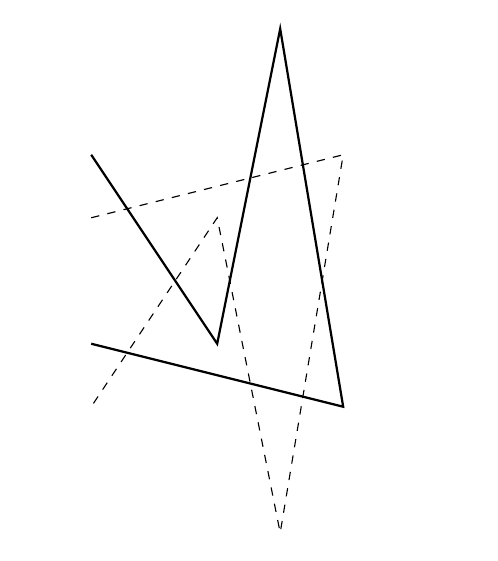
\begin{tikzpicture}[scale=0.8]
            \def\mypath{(-2,-1) -- (2,-2) --(1,4) -- (0,-1)--(-2,2)}
            \draw [white](-3,-3) grid (4,4);
            \draw [thick]\mypath ;
            %\draw (-2,-2)--(3,3) node [right]{$(d)$} ;
            \draw [dashed,cm={1,0,0,-1,(0,0)}] \mypath;%Matrice de transformation inverse X et Y
        \end{tikzpicture}
    \end{figure}
\end{minipage}

\textbf{Pour les exercices \ref{CentreSymCent1} à \ref{CentreSymCent4} :} Trouver le centre qui permet les symétrie centrales suivantes.

\begin{minipage}[t]{0.45\textwidth}
    \exo{Représenter}{CentreSymCent1}
    
    \begin{figure}[H]
        \centering
        \begin{tikzpicture}[scale=0.8]
            \tikzset{
                homothety at/.style args={#1 scaled by #2}{shift={($(#1)!#2!(0,0)$)},scale=#2},}
            \def\mypath{(-2,-2) -- (-1,1) --(-2,0) -- (-1,1.5)--(0,0)--(-2,-2)}
            \draw [white](-3,-3) grid (4,4);
            \fill[white] (0,0) coordinate (c) circle(2pt) node [above] {$O$};
            \draw [thick]\mypath ;
            \begin{scope}[homothety at=c scaled by -1]
                \draw [dashed]\mypath;
            \end{scope}
        \end{tikzpicture}
    \end{figure}
\end{minipage}
\hfill
\begin{minipage}[t]{0.45\textwidth}
    \exo{Représenter}{CentreSymCent2}
    
    \begin{figure}[H]
        \centering
        \begin{tikzpicture}[scale=0.8]
            \tikzset{
                homothety at/.style args={#1 scaled by #2}{shift={($(#1)!#2!(0,0)$)},scale=#2},}
            \def\mypath{(-3,2) -- (-1,1) --(0,2) -- (1,3)--(0,1)--(-2,2)}
            \fill[white] (1,0) coordinate (c) circle(2pt) node [above] {$O$};
            \draw [white](-3,-3) grid (4,4);
            \draw [thick]\mypath ;
            \begin{scope}[homothety at=c scaled by -1]
                \draw[dashed] \mypath;
            \end{scope}
        \end{tikzpicture}
    \end{figure}
\end{minipage}

\begin{minipage}[t]{0.45\textwidth}
    \exo{Représenter}{CentreSymCent3}
    
    \begin{figure}[H]
        \centering
        \begin{tikzpicture}[scale=0.8]
            \tikzset{
                homothety at/.style args={#1 scaled by #2}{shift={($(#1)!#2!(0,0)$)},scale=#2},}
            \def\mypath{(1,-2) -- (0,-1) --(3,-2) -- (2,-1)--(-1,-1)--(1,-2)}
            \fill [white](0,0) coordinate (c) circle(2pt) node [above] {$O$};
            \draw [white](-3,-3) grid (4,4);
            \draw [thick]\mypath ;
            \begin{scope}[homothety at=c scaled by -1]
                \draw [dashed]\mypath;
            \end{scope}
        \end{tikzpicture}
    \end{figure}
\end{minipage}
\hfill
\begin{minipage}[t]{0.45\textwidth}
    \exo{Représenter}{CentreSymCent4}
    
    \begin{figure}[H]
        \centering
        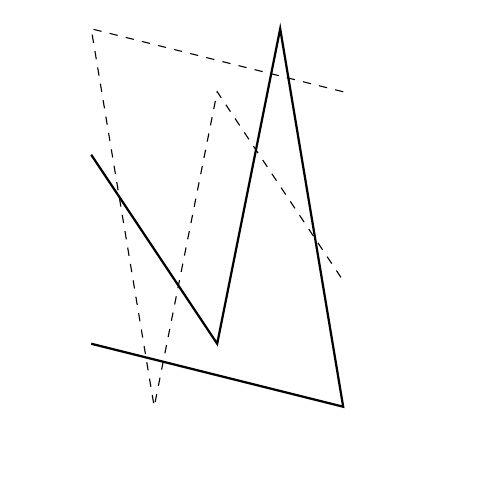
\begin{tikzpicture}[scale=0.8]
            \tikzset{
                homothety at/.style args={#1 scaled by #2}{shift={($(#1)!#2!(0,0)$)},scale=#2},}
            \def\mypath{(-2,-1) -- (2,-2) --(1,4) -- (0,-1)--(-2,2)}
            \fill [white](0,1) coordinate (c) circle(2pt) node [above] {$O$};
            \draw [white](-3,-3) grid (4,4);
            \draw [thick]\mypath ;
            \begin{scope}[homothety at=c scaled by -1]
                \draw [dashed]\mypath;
            \end{scope}
        \end{tikzpicture}
    \end{figure}
\end{minipage}

\newpage
\textbf{Pour les exercices \ref{CentreRota1} à \ref{CentreRota4} :} Trouver le centre et l'angle  des rotations suivantes.
\vspace{-2em}

\begin{minipage}[t]{0.45\textwidth}
    \exo{Représenter}{CentreRota1}
        
    \begin{figure}[H]
        \centering
        \begin{tikzpicture}[scale=0.8]
            \def\mypath{(-2,-2) -- (-1,1) --(-2,0) -- (-1,1.5)--(0,0)--(-2,-2)}
            \fill[white] (0,0) coordinate (c) circle(2pt) node [above] {$0$};
            \draw [white](-3,-3) grid (4,4);
            \draw [thick]\mypath ;
            \draw [dashed,rotate=-160] \mypath ;
        \end{tikzpicture}
    \end{figure}
\end{minipage}
\hfill
\begin{minipage}[t]{0.45\textwidth}
    \exo{Représenter}{CentreRota2}
        
    \begin{figure}[H]
        \centering
        \begin{tikzpicture}[scale=0.8]
            \def\mypath{(-3,2) -- (-1,1) --(0,2) -- (1,3)--(0,1)--(-2,2)}
            \fill[white] (0,0) coordinate (c) circle(2pt) node [above] {$0$};
            \draw [white](-3,-3) grid (4,4);
            \draw [thick]\mypath ;
            \draw [dashed,rotate=30] \mypath ;
        \end{tikzpicture}
    \end{figure}
\end{minipage}

\begin{minipage}[t]{0.45\textwidth}
    \exo{Représenter}{CentreRota3}
        
    \begin{figure}[H]
        \centering
        \begin{tikzpicture}[scale=0.8]
            \def\mypath{(1,-2) -- (0,-1) --(3,-2) -- (2,-1)--(-1,-1)--(1,-2)}
            \fill[white] (0,0) coordinate (c) circle(2pt) node [above] {$0$};
            \draw [white](-3,-3) grid (4,4);
            \draw [thick]\mypath ;
            \draw [dashed,rotate=-75] \mypath ;
        \end{tikzpicture}
    \end{figure}
\end{minipage}
\hfill
\begin{minipage}[t]{0.45\textwidth}
    \exo{Représenter}{CentreRota4}
        
    \begin{figure}[H]
        \centering
        \begin{tikzpicture}[scale=0.8]
            \def\mypath{(-2,-1) -- (2,-2) --(1,4) -- (0,-1)--(-2,2)}
            \fill[white] (0,0) coordinate (c) circle(2pt) node [above] {$0$};
            \draw [white](-3,-3) grid (4,4);
            \draw [thick]\mypath ;
            \draw [dashed,rotate=110] \mypath ;
        \end{tikzpicture}
    \end{figure}
\end{minipage}
\vspace{1em}
\textbf{Pour les exercices \ref{CentreHomot1} à \ref{CentreHomot4} :}Trouver le centre et le rapport des homotéties suivantes.
\vspace{-2em}

\begin{minipage}[t]{0.45\textwidth}
    \exo{Représenter}{CentreHomot1}
        
    \begin{figure}[H]
        \centering
        \begin{tikzpicture}[scale=0.8]
            \tikzset{
                homothety at/.style args={#1 scaled by #2}{shift={($(#1)!#2!(0,0)$)},scale=#2},}
            \fill[white] (-1,-1) coordinate (c) circle(2pt) node [above] {$O$};
            \def\mypath{(-2,-2) -- (-1,1) --(-2,0) -- (-1,1.5)--(0,0)--(-2,-2)}
            \draw [white](-3,-3) grid (5,5);
            \draw [thick]\mypath ;
            \begin{scope}[homothety at=c scaled by 2]
                \draw[dashed] \mypath;
            \end{scope}
        \end{tikzpicture}
    \end{figure}
\end{minipage}
\hfill
\begin{minipage}[t]{0.45\textwidth}
    \exo{Représenter}{CentreHomot2}
        
    \begin{figure}[H]
        \centering
        \begin{tikzpicture}[scale=0.8]
            \tikzset{
                homothety at/.style args={#1 scaled by #2}{shift={($(#1)!#2!(0,0)$)},scale=#2},}
            \def\mypath{(-3,2) -- (-1,1) --(0,2) -- (1,3)--(0,1)--(-2,2)}
            \draw [white](-3,-3) grid (5,5);
            \draw [thick]\mypath ;
            \fill[white] (0,-2) coordinate (c) circle(2pt) node [above] {$O$};
            \begin{scope}[homothety at=c scaled by 0.75]
                \draw[dashed] \mypath;
            \end{scope}
        \end{tikzpicture}
    \end{figure}
\end{minipage}

\begin{minipage}[t]{0.45\textwidth}
    \exo{Représenter}{CentreHomot3}
        
    \begin{figure}[H]
        \centering
        \begin{tikzpicture}[scale=0.8]
            \tikzset{
                homothety at/.style args={#1 scaled by #2}{shift={($(#1)!#2!(0,0)$)},scale=#2},}
            \def\mypath{(-1,-2) -- (0,-1) --(3,-2) -- (2,0)--(-1,-3)--(-1,-2)}
            \draw [white](-3,-3) grid (5,5);
            \draw [thick]\mypath ;
            \fill[white] (1,0) coordinate (c) circle(2pt) node [above] {$O$};
            \begin{scope}[homothety at=c scaled by -2]
                \draw[dashed] \mypath;
            \end{scope}
        \end{tikzpicture}
    \end{figure}
\end{minipage}
\hfill
\begin{minipage}[t]{0.45\textwidth}
    \exo{Représenter}{CentreHomot4}
        
    \begin{figure}[H]
        \centering
        \begin{tikzpicture}[scale=0.8]
            \tikzset{
                homothety at/.style args={#1 scaled by #2}{shift={($(#1)!#2!(0,0)$)},scale=#2},}
            \def\mypath{(-1,-1) -- (2,-2) --(1,3) -- (0,-1)--(-1,2)}
            \draw [white](-3,-3) grid (5,5);
            \draw [thick]\mypath ;
            \fill[white] (2,1) coordinate (c) circle(2pt) node [above] {$O$};
            \begin{scope}[homothety at=c scaled by 1.5]
                \draw[dashed] \mypath;
            \end{scope}
        \end{tikzpicture}
    \end{figure}
\end{minipage}

\newpage

\exo{Modéliser}{Dur1}
On considère un triangle $ABC$ quelconque. On appelle :
\begin{itemize}
    \item $D$ l'image de $A$ par la symétrie de centre $A$
    \item $E$ l'image de $B$ par la symétrie de centre $A$
    \item $F$ l'image de $C$ par la symétrie de centre $A$
    \item $G$ l'image de $A$ par la symétrie de centre $B$
    \item $H$ l'image de $B$ par la symétrie de centre $B$
    \item $I$ l'image de $C$ par la symétrie de centre $B$
    \item $J$ l'image de $D$ par la symétrie de centre $E$
    \item $K$ l'image de $E$ par la symétrie de centre $E$
    \item $L$ l'image de $F$ par la symétrie de centre $E$
\end{itemize}

Quels sont les points occupant la même position ?

\exo{Chercher}{Dur2}
    
Si $(d)$ est une droite et $(d')$ son image par une symétrie axiale, à quelle condition est-ce que $(d)$ et $(d')$ sont parallèles ?




%Ce qu'il faut imprimer pour les élèves
%Penser à retirer le comment du \nofile dans le main ligne 32




\rhead{Devoir n° 1 du 29 Septembre 2023}


\lhead{Nom, prénom :}

\exo{4}{Calculer} Calculer en détaillant les étapes

\begin{multicols}{2}
    $$-13-14$$
    \vspace*{3em}

    $$-12+21$$
    \vspace*{7em}\columnbreak

    $$-6+4-12+2$$
    \vspace*{3em}

    $$-12+11-14+20+3$$
    \vspace*{7em}
\end{multicols}

\vspace*{-1em}

\exo{4}{Calculer} Calculer en détaillant les étapes

\begin{multicols}{2}
    $$(+12)+(-11)+(-6)+(+1)$$
    \vspace*{8em}

    $$(-10)-(-5)+(-8)-(+5)$$
    \vspace*{8em}\columnbreak

    $$(-1)-(-1)+(-6)+(-1)-(+8)-(-5)$$
    \vspace*{8em}

    $$(+6)-(+3)-(-8)-(+4)-(-3)-(+6)$$
    \vspace*{8em}
\end{multicols}

\newpage



\exo{4}{Chercher} Trouve les erreurs :

\begin{multicols}{2}
    \noindent\begin{align*}
        &(+10)+(-6)-(+2)-(-12)\\
        =&+10-6-2-12\\
        =&+10-20\\
        =&-10
    \end{align*}

    \noindent\begin{align*}
        &(-13)-(-4)-(+5)+(+9)\\
        =&-13+4-5+9\\
        =&-18+13\\
        =&+5
    \end{align*}

\end{multicols}

\exo{4}{Modéliser} Résoudre les problèmes suivants :

\begin{minipage}{0.45\textwidth}
    Crabe et Goyle jouent à un jeu de société. Crabe a 12 points et Goyle en a 27.
    Crabe lui échange un jeton valant -5 points contre un jeton en valant +3. 
    Qui a le plus de point désormais ?
    \vspace*{8em}
\end{minipage}
\hfil
\vrule
\hfil
\begin{minipage}{0.45\textwidth}
    Crabe et Goyle jouent à un jeu de société. Crabe a -12 points et Goyle en a -1.
    Crabe lui échange un jeton valant -4 points contre un jeton en valant +1. 
    Qui a le plus de point désormais ?
    \vspace*{8em}
\end{minipage}

\exo{4}{Raisonner} Simplifier les écritures suivantes.

\begin{multicols}{2}
    $$-(+(-5))$$
    \vspace*{3em}

    $$-(-(+(-7)))$$
    \vspace*{7em}\columnbreak

    $$+(+(-1))$$
    \vspace*{3em}

    $$+(-(-(+2)))$$
    \vspace*{7em}
\end{multicols}

\exo{}{Calculer}

$$6\times 5 -(-4-(-2))\times 3 +((9\times 4)-(-6))\div 7+\noindent4-(+12)$$


\newpage

\setcounter{exrcntr}{0}

\exrc (4 points) Effectuer les calculs suivants

\begin{tabularx}{\textwidth}{Y|Y}
    \cnt  & \cnt  \\
    $3+5\times 7 -3+1$ & $4+5\times (6-3+2)$
\end{tabularx} 

\exrc (2 points) Compléter le tableau suivant \textbf{(peut être fait sur le sujet)}.

\begin{tabularx}{\textwidth}{Y|Y}
    Forme décimale & Forme pourcentage \\ \hline
    & 35\% \\ \hline
    0,65 & \\ \hline
    & 9\% \\ \hline
    0,8 & 
\end{tabularx} 

\exrc (4 points) A l'aide du diagrame ci dessous.

\begin{figure}[H]
    \centering
    \begin{tikzpicture}
    \draw[ultra thick,->] (0,0)--(6,0) ; 
    \draw[ultra thick,->] (0,0) -- (0,4) ; 
    \foreach \r in {1,...,5}{\draw[color=black] (\r , -0.1)--(\r , 0.1);
    \draw (\r , -0.3) node {\r} ;}
    \foreach \r in {1,...,3}{\draw[color=black] (-0.1,\r )--( 0.1, \r);
    \draw (-0.3 , \r) node {\r} ;}
    \draw[thick] (1,0) -- (1,2) ;
    \draw[thick] (2,0) -- (2,3) ;
    \draw[thick] (3,0) -- (3,1) ;
    \draw[thick] (4,0) -- (4,2) ;
    \draw[thick] (5,0) -- (5,2) ;
    \end{tikzpicture}
    \end{figure}

\cnt (2 points) Compléter le tableau d'effectif \textbf{(peut être fait sur le sujet)}.

\begin{tabularx}{\textwidth}{Y*{5}{|Y}}
    Valeur &  1 & 2 & 3 & 4 & 5\\ \hline
    Effectif &  &  &  & &
\end{tabularx} 

\cnt (1 point) Calculer la fréquence de la valeur 5.

\cnt (1 point) Calculer la fréquence de la valeur 3.

\newpage

\exrc (5 points) Calculer les moyennes des séries suivantes

\cnt (2 points) 1 ; 2 ; 3 ; 4 ; 10 

\cnt (2 points) 5 ; 11 ; 14 ; 8 ; 13 ; 9

\cnt (1 points) la série définie par le tableau suivant :

\begin{tabularx}{\textwidth}{Y*{4}{|Y}}
    Valeur &  2 & 4 & 5 & 10\\ \hline
    Effectif & 3 & 1 & 2 & 4
\end{tabularx} 

\exrc (5 points) Calculer les médianes des séries suivantes

\cnt (2 points) 1 ; 2 ; 3 ; 4 ; 5 

\cnt (2 points) 12 ; 13 ; 7 ; 5 ; 1 ; 2

\cnt (1 points) la série définie par le tableau suivant :

\begin{tabularx}{\textwidth}{Y*{5}{|Y}}
    Valeur &  12 & 15  & 19 & 25 & 39\\ \hline
    Effectif & 2 & 1 & 1 & 4 & 3
\end{tabularx} 

\makeatletter
\newcounter{int}
\@whilenum\value{int}<\value{repetition}\do
{\stepcounter{int}\vspace{0.3cm}\setcounter{propcntr}{0}\setcounter{excntr}{0}
\rhead{Devoir n° 1 du 29 Septembre 2023}


\lhead{Nom, prénom :}

\exo{4}{Calculer} Calculer en détaillant les étapes

\begin{multicols}{2}
    $$-13-14$$
    \vspace*{3em}

    $$-12+21$$
    \vspace*{7em}\columnbreak

    $$-6+4-12+2$$
    \vspace*{3em}

    $$-12+11-14+20+3$$
    \vspace*{7em}
\end{multicols}

\vspace*{-1em}

\exo{4}{Calculer} Calculer en détaillant les étapes

\begin{multicols}{2}
    $$(+12)+(-11)+(-6)+(+1)$$
    \vspace*{8em}

    $$(-10)-(-5)+(-8)-(+5)$$
    \vspace*{8em}\columnbreak

    $$(-1)-(-1)+(-6)+(-1)-(+8)-(-5)$$
    \vspace*{8em}

    $$(+6)-(+3)-(-8)-(+4)-(-3)-(+6)$$
    \vspace*{8em}
\end{multicols}

\newpage



\exo{4}{Chercher} Trouve les erreurs :

\begin{multicols}{2}
    \noindent\begin{align*}
        &(+10)+(-6)-(+2)-(-12)\\
        =&+10-6-2-12\\
        =&+10-20\\
        =&-10
    \end{align*}

    \noindent\begin{align*}
        &(-13)-(-4)-(+5)+(+9)\\
        =&-13+4-5+9\\
        =&-18+13\\
        =&+5
    \end{align*}

\end{multicols}

\exo{4}{Modéliser} Résoudre les problèmes suivants :

\begin{minipage}{0.45\textwidth}
    Crabe et Goyle jouent à un jeu de société. Crabe a 12 points et Goyle en a 27.
    Crabe lui échange un jeton valant -5 points contre un jeton en valant +3. 
    Qui a le plus de point désormais ?
    \vspace*{8em}
\end{minipage}
\hfil
\vrule
\hfil
\begin{minipage}{0.45\textwidth}
    Crabe et Goyle jouent à un jeu de société. Crabe a -12 points et Goyle en a -1.
    Crabe lui échange un jeton valant -4 points contre un jeton en valant +1. 
    Qui a le plus de point désormais ?
    \vspace*{8em}
\end{minipage}

\exo{4}{Raisonner} Simplifier les écritures suivantes.

\begin{multicols}{2}
    $$-(+(-5))$$
    \vspace*{3em}

    $$-(-(+(-7)))$$
    \vspace*{7em}\columnbreak

    $$+(+(-1))$$
    \vspace*{3em}

    $$+(-(-(+2)))$$
    \vspace*{7em}
\end{multicols}

\exo{}{Calculer}

$$6\times 5 -(-4-(-2))\times 3 +((9\times 4)-(-6))\div 7+\noindent4-(+12)$$


\newpage

\setcounter{exrcntr}{0}

\exrc (4 points) Effectuer les calculs suivants

\begin{tabularx}{\textwidth}{Y|Y}
    \cnt  & \cnt  \\
    $3+5\times 7 -3+1$ & $4+5\times (6-3+2)$
\end{tabularx} 

\exrc (2 points) Compléter le tableau suivant \textbf{(peut être fait sur le sujet)}.

\begin{tabularx}{\textwidth}{Y|Y}
    Forme décimale & Forme pourcentage \\ \hline
    & 35\% \\ \hline
    0,65 & \\ \hline
    & 9\% \\ \hline
    0,8 & 
\end{tabularx} 

\exrc (4 points) A l'aide du diagrame ci dessous.

\begin{figure}[H]
    \centering
    \begin{tikzpicture}
    \draw[ultra thick,->] (0,0)--(6,0) ; 
    \draw[ultra thick,->] (0,0) -- (0,4) ; 
    \foreach \r in {1,...,5}{\draw[color=black] (\r , -0.1)--(\r , 0.1);
    \draw (\r , -0.3) node {\r} ;}
    \foreach \r in {1,...,3}{\draw[color=black] (-0.1,\r )--( 0.1, \r);
    \draw (-0.3 , \r) node {\r} ;}
    \draw[thick] (1,0) -- (1,2) ;
    \draw[thick] (2,0) -- (2,3) ;
    \draw[thick] (3,0) -- (3,1) ;
    \draw[thick] (4,0) -- (4,2) ;
    \draw[thick] (5,0) -- (5,2) ;
    \end{tikzpicture}
    \end{figure}

\cnt (2 points) Compléter le tableau d'effectif \textbf{(peut être fait sur le sujet)}.

\begin{tabularx}{\textwidth}{Y*{5}{|Y}}
    Valeur &  1 & 2 & 3 & 4 & 5\\ \hline
    Effectif &  &  &  & &
\end{tabularx} 

\cnt (1 point) Calculer la fréquence de la valeur 5.

\cnt (1 point) Calculer la fréquence de la valeur 3.

\newpage

\exrc (5 points) Calculer les moyennes des séries suivantes

\cnt (2 points) 1 ; 2 ; 3 ; 4 ; 10 

\cnt (2 points) 5 ; 11 ; 14 ; 8 ; 13 ; 9

\cnt (1 points) la série définie par le tableau suivant :

\begin{tabularx}{\textwidth}{Y*{4}{|Y}}
    Valeur &  2 & 4 & 5 & 10\\ \hline
    Effectif & 3 & 1 & 2 & 4
\end{tabularx} 

\exrc (5 points) Calculer les médianes des séries suivantes

\cnt (2 points) 1 ; 2 ; 3 ; 4 ; 5 

\cnt (2 points) 12 ; 13 ; 7 ; 5 ; 1 ; 2

\cnt (1 points) la série définie par le tableau suivant :

\begin{tabularx}{\textwidth}{Y*{5}{|Y}}
    Valeur &  12 & 15  & 19 & 25 & 39\\ \hline
    Effectif & 2 & 1 & 1 & 4 & 3
\end{tabularx} }
\makeatother

\end{document}
